\documentclass[11pt,a4paper]{article}

\usepackage{geometry} \geometry{left=2.2cm, right=2.2cm, top=2.2cm, bottom=2cm}
\parskip 0.15cm 
\setlength{\parindent}{0cm} 
\usepackage{pdflscape}
\usepackage[document]{ragged2e}

\usepackage[T1]{fontenc}  % Set font

\usepackage{lineno}  % Line numbers

\usepackage{amssymb}  % Symbols
\usepackage{amsmath}

\linespread{1.25}  % Linespacing

\usepackage{xcolor} \newcommand{\todo}[1]{\textcolor{red}{\textbf{#1}}}   %

% Tables
\usepackage{multirow} \setlength{\tabcolsep}{4pt}

% Image handling
\usepackage{graphicx} 

\makeatletter \g@addto@macro\@floatboxreset\centering  
\makeatother

\graphicspath{ {img/} }  % Define image path

\usepackage{subfig}  % Compound figures

\usepackage{float}  % Precise figure location

% Bibliography management
\usepackage[style=authoryear, natbib=true, backend=biber]{biblatex}
\addbibresource{workflow.bib}

% Links within document, nice figure formatting
\usepackage[breaklinks]{hyperref} \definecolor{links}{RGB}{0,0,0} \hypersetup{
	breaklinks, colorlinks=true, linkcolor=links, anchorcolor=links,
	citecolor=links, filecolor=links, menucolor=links, runcolor=links,
	urlcolor=links, pdfauthor={John L. Godlee} }
	\def\subsectionautorefname{section} \def\subsubsectionautorefname{section}

\newcommand{\beginsupplement}{% 
	\setcounter{table}{0}
	\renewcommand{\thetable}{S\arabic{table}}% 
	\setcounter{figure}{0}
	\renewcommand{\thefigure}{S\arabic{figure}}% 
}
     
% Variables
\newcommand{\titletext}{Terrestrial LiDAR processing workflow}

% Body
\begin{document}

{\Large{Title: \titletext{}}}

\section{Introduction}

This document details the processing workflow for the terrestrial LiDAR data collected during fieldwork in Bicuar National Park, Angola, and Kilwa District, Tanzania, with the aim of documenting a reproducible workflow.

The project aimed to understand the effects of tree species diversity and composition on tree canopy architecture and grassy biomass.

\section{Field methods}

Fieldwork was conducted at two sites, the first in Bicuar National Park, southwest Angola (LATLONG), and the second in Kilwa District, southeast Tanzania (LATLOPNG). 

The two sites have similar climatic conditions.

TABLE OF CLIMATE

Fieldwork was conducted during the peak growth period of each site, in order to capture the highest leafy volume in the canopy and the largest grassy volume in the understorey.

At each site, 1 ha permanent plots were sampled. In Angola, 15 plots were used, while in Tanzania, only seven were used, following the curtailment of fieldwork due to COVID-19 travel restrictions.

Each permanent plot was further subdivided into nine 10 m diameter circular subplots arranged in a regular grid, with a buffer from the plot edge (FIGURE).

Within each subplot, a variable number of scans were recorded using a Leica HDS6100 phase-shift terrestrial laser scanner (TLS). The number and position of scans within a subplot was determined by the arrangement and density of canopy material in the subplot. Scan positions were arranged to minimise shadows within the canopy, and to maximise canopy penetration. Number of scans per subplot ranged between one and five in both Angola and Tanzania (\autoref{scan_settings}).

Five Leica 6" planar tilt and turn targets were used at each subplot to align scans. To allow for registration of scans among subplots, the location of each target was registered using a Leica VIVA GS10 GNSS unit, set up in post-processed kinematic (PPK) configuration with a base-station located \textasciitilde{}100 m from the edge of each 1 ha plot. The location of each target was measured for at least 4 minutes. MORE ABOUT DIALLING IN THE GNSS values. 


\begin{table}[H] \centering 
  \caption{Description of scan settings used for each scan.} 
  \label{scan_settings} 
\begin{tabular}{@{\extracolsep{0pt}} rl} 
\\[-1.8ex]\hline 
\hline \\[-1.8ex] 
{Setting} & {Value} \\
\hline \\[-1.8ex] 
Scanner model & Leica HDS6100 \\
Wavelength & 650-690 nm \\
Spot size at exit & 3 mm \\
Beam divergence & 0.22 mrad \\
Range & 79 m @90\%; 50 m @18\% albedo \\
Azimuth range & 0-360\textdegree{} \\
Zenith range & 0-155\textdegree{} \\
Increments & 0.018\textdegree{} \\
Point spacing over 25 m & 7.9 mm \\
Pixels per line & 20000 \\
Lines & 10000 \\
Compressed file size & \textasciitilde{}800 MB \\
Duration of scan & 6 minutes 44 seconds \\
\hline
\hline \\[-1.8ex] 
\end{tabular} 
\end{table} 

\begin{figure}[H]
\centering
	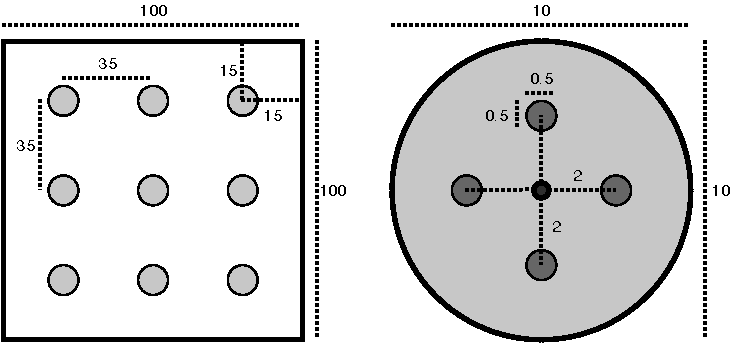
\includegraphics[width=\textwidth]{subplot}
	\caption{The layout of 10 m diameter subplots with each larger 1 ha square plot. Each subplot is situated inside a 15 m buffer from the plot edge, with 35 m between subplot centres. Subplots are arranged in a 3x3 grid. Disc-pasture measurements and biomass samples are located in cardinal directions 2 m from the centre of the subplot. All distances are in metres.}
	\label{subplot}
\end{figure}


\section{Registration}

Scan registration for each subplot was conducted in Leica Cyclone version XXXX. Targets from each scan were aligned using Cyclone's automatic target acquisition. 

We used SOME KIND OF GLOBAL SATELLITE MATCHING TO MAKE THE GNSS BETTER.

After registration, scan scenes were exported from Cyclone as PTX files, one per subplot.

\section{Voxelization}

PTX files were converted to compressed LAZ files using PDAL \citep{}. The exact code used to extract and apply the PTX rotation matrix to each point in the PTX file can be found IN THIS APPENDIX HERE. 

LAZ files were voxelised to different voxel sizes depending on the application of the data. For grassy biomass estimation, I used XXX cm\textsuperscript{3} cubic voxels, while for subplot height profile estimation I used XXX cm\textsuperscript{3} voxels, and for whole plot canopy rugosity I used XXX cm\textsuperscript{3} voxels. WHY THO

\section{Noise reduction}

Outlier detection and noise reduction was conducted in PDAL using the \texttt{filters.outlier} filter, using the ``statistical method'' (sensu \citealt{Rusu2008}), with $k = 8$ (mean number of neighbours), and $m = 1.96$ (standard deviation threshold, approximating a 95\% confidence interval):

\begin{align}
	\overline{\mu} &= \frac{1}{N} \sum_{i=1}^{N} \mu_{i} \\
	\sigma &= \sqrt{\frac{1}{N-1} \sum_{i=1}^{N}(\mu_{i} - \overline{\mu{}})^2} \\
	t &= \mu + m \sigma \\
	\text{outlier}_{i} &= 
		\begin{cases}
			\text{true}, & \text{if}\ \mu_{i} >= t \\
			\text{false}, & \text{otherwise}
		\end{cases}
\end{align}

where $N$ is the number of points in the scene, $\overline{\mu}$ is the mean distance to nearest neighbour points, and $\sigma$ is the standard deviation of these distances. $t$ is the threshold distance used to define an outlier.

\section{Foliage density profiles}

To estimate subplot foliage density profiles, first the point cloud was cropped to a 10 m diameter cylinder of infinite height. Then the \texttt{filters.pmf} (Progressive Morphological Filter - PMF) PDAL function was used to identify ground points (sensu \citealt{Zhang2003}). The \texttt{filters.hag\_nn} (Nearest Neighbour) PDAL function was used to generate height above ground of each point within the cylinder. Points below ground level were then discarded. Height profile points were exported to a XYZ file then imported into R for further processing. 

We excluded points above the 99.9th percentile of height, under the assumption that these often constituted noise that had not been adequately removed by PDAL.

In R, within each 1 cm width vertical layer, we calculated the gap fraction as the proportion of unfilled 1 cm\textsuperscript{3} voxels. We filtered the point cloud data to the tree canopy, excluding grass. We identified the breakpoint between the grassy understorey and the tree canopy as the first local minima above 1.3 m from the ground. 

We extracted statistics from the foliage density profile for use in statistical analysis. We first smoothed the density profile using a loess model with a span of 0.1. We then calculated the number of local maxima and minima along the profile. We defined local maxima and minima as points regions where the gap fraction of the surrounding 50 cm of 1 cm bins was lower or higher, respectively.

We calculated the effective number of layers (ENL), using the Shannon diversity index (sensu \citep{Ehbrecht2016}). 

We calculated the area under the curve of foliage density using trapezoid estimation.

We extracted the height of the maximum foliage density peak, and calculated the difference between the highest and lowest local maxima. We also extracted the maximum canopy height within the subplot.

We calculated the coefficient of variation of the point cloud height distribution.

To describe the uniformity of the foliage density distribution we used Ripley's L function, which is more commonly used in describing spatial variation across a 2 dimensional surface. Ripley's L is an adjustment to Ripley's K, defined as:

\begin{align}
	\widehat{K}(t) &= \lambda^{-1} \sum_{i\neq{}j} \frac{I(d_{ij} < t)}{n} \\
	\widehat{L}(t) &= \left(\frac{\widehat{K}(t)}{\pi}\right)^{1/2}
\end{align}

Finally, we calculated the Shannon diversity index on gap fraction of 50 cm bins

\section{Canopy gap fraction}

\section{Grassy biomass estimation}

\section{Canopy rugosity}

\printbibliography

\end{document}

